\documentclass[a4paper]{article}
\usepackage[portuguese]{babel}
\usepackage[latin1]{inputenc}
\usepackage[T1]{fontenc}
\usepackage{fancyvrb}
\usepackage{url}
\usepackage{graphicx}
\usepackage{float}
\usepackage[affil-it]{authblk}
\usepackage{indentfirst}
 
\usepackage{titlesec}
 
\usepackage{aeguill} % usefull for pdflatex
\usepackage[compat2,a4paper,twosideshift=0mm,left=20mm,right=20mm,bottom=20mm,top=15mm]{geometry}
 
\parindent=2em
 
\usepackage{xcolor}
\usepackage{listings}
 
 
\lstdefinestyle{gramatica}{
backgroundcolor=\color{yellow!7},%
numbers=left, numberstyle=\tiny, stepnumber=1, numbersep=5pt,%
basicstyle=\small\ttfamily\color{blue},%
breaklines=true,% allow line breaks
moredelim=[s][\color{green!50!black}\ttfamily]{'}{'},% single quotes in green
moredelim=*[s][\color{black}\ttfamily]{options}{\}},% options in black (until trailing })
commentstyle={\color{gray}\itshape},% gray italics for comments
morecomment=[l]{//},% define // comment
emph={%
STRING% literal strings listed here
},emphstyle={\color{blue}\ttfamily},% and formatted in blue
alsoletter={:,|,;},%
morekeywords={:,|,;},% define the special characters
keywordstyle={\color{black}},% and format them in black
}
 
 
 
 
\title{Exercí­cio para Avaliação n.º 3}
\author{Bruno Azevedo%
\thanks{Email: \texttt{azevedo.252@gmail.com}}}
 
\author{Miguel Costa%
\thanks{Email: \texttt{miguelpintodacosta@gmail.com}}}
 
\affil{Módulo Engenharia Gramatical,\\ UCE30 Engenharia de Linguagens,
\\ Mestrado em Engenharia Informatica,\\Universidade do Minho}
 
 
\date{\today}
 
 
\begin{document}
 
 
\maketitle
 
\begin{abstract}
Este documento apresenta a resolução do Exercício Prático n.º 3 do módulo de Engenharia Gramatical.
O exercício está relacionado com a geração automática de Processadores de Linguagens a partir de Gramáticas.
 
Era pretendido criar uma linguagem para fazer movimentar um Robo num Terreno e depois criar um processador para as frases da linguagem com algumas funcionalidades.
\end{abstract}
 
 
\newpage
 
\parskip=0mm
\tableofcontents
\parskip=2mm
 
\newpage
 
\section{Ambiente de Trabalho}
Foi necessário usar um Gerador de Compiladores para gerar o nosso próprio compilador, por isso usámos o AnTLR que é também usado nas aulas. Para facilitar o processo de debugging durante a resolução do problema dado, usámos a ferramenta AnTLRWorks, que tem uma interface bastante agradável e simpática para ajudar a resolver problemas desta natureza.
 
A linguem de programação adoptada foi o JAVA. De forma tornar a nossa solução mais legível e estruturada, criámos classes com o auxílio do IDE NetBeans que nos ajudou no desenvolvimento do código JAVA e ainda na criação da sua documentação (javadoc).
 
 
\section{Descrição do problema}
Imaginemos um robo com a função de aspirar um terreno de forma retangular. Este terreno tem uma área que é conhecida pelo robo e que acaba por limitar o raio de ação dele.
 
O robo pode ter definida uma posição inicial e os seus movimentos podem ser em quatro direções diferentes (norte, sul, este e oeste) com um peso associado que representa a distância que se vai deslocar (por exemplo \verb|NORTE 4|, desloca-se 4 unidades para norte). Tem ainda a opção de estar ligado ou desligado que define se está ativo ou não para aspirar.
 
Com base na descrição do robo, era pedido:
\begin{enumerate}
\item Criar uma linguagem que conseguisse descrever uma rotina possível para o robo. Esta linguagem deve permitir ainda que tenha no início certas definições como a dimensão do terreno e a posição inicial do robo.
\item Depois de definida a linguagem, tínhamos de criar um processador para as possíveis frases que podiam ser geradas com as seguintes funcionalidades:
\begin{itemize}
\item Verificar que o robo não se movimenta para fora da área de limpeza.
\item Calcular a distância (em cm) que o robo percorreu durante a sua rotina.
\item Determinar quantas mudanças de direção foram feitas pelo robo.
\item Determinar a distância média que o robo se desloca por cada movimento.
\end{itemize}
\end{enumerate}
 
 
\section{Criação da linguagem}
Analisando o que era pretendido para descrever a rotina do robo, tentámos criar uma linguagem com uma sintaxe de fácil leitura e sem ambiguidades. Depois de analisar várias alternativas, definimos a linguagem com a seguinte estrutura:
\lstset{caption={Estrutura da gramática},label=DescriptiveLabel}
\begin{lstlisting}[style=gramatica]
ASPIRADOR
{
DEFINICOES
{
definicao1; definicao2;
}
MOVIMENTOS
instrucao1;
instrucao2;
....
}
\end{lstlisting}
 
Uma linguagem tem de ter símbolos terminais e neste caso definimos os símbolos:
\begin{itemize}
\item DIM
\item POS
\item LIGAR
\item DESLIGAR
\item NORTE
\item SUL
\item ESTE
\item OESTE
\item ID
\item INT
\end{itemize}
 
Definindo formalmente a gramática para representar os eventos possíveis do robo, obtemos:
\lstset{caption={Gramática},label=DescriptiveLabel}
\lstinputlisting[style=gramatica]{gramatica.g}
 
Depois de gerada a gramática, uma frase que se pode gerar é:
\lstset{caption={Frase gerada 1},label=DescriptiveLabel}
\lstinputlisting[style=gramatica]{in1.txt}
Para provar que era uma frase válida, fizemos a sua árvore de derivação:
\begin{figure}[H]
\centering
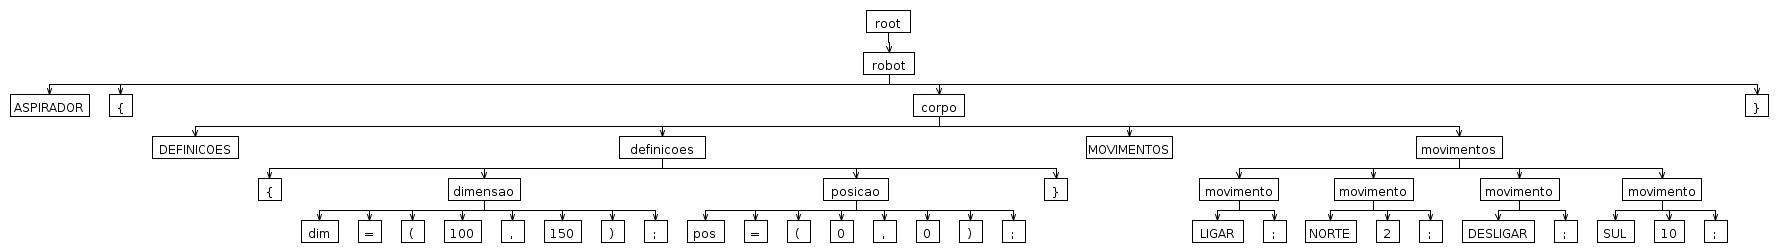
\includegraphics[scale=0.29]{arv1.jpeg}
% imag2.png: 688x477 pixel, 72dpi, 24.27x16.83 cm, bb=0 0 688 477
\caption{Árvore de derivação}
\end{figure}
 
 
Analisando a gramática a as frases geradas a partir dela, verificámos que o elemento raiz é \verb|robot| e o parser terá de encontrar, no início, a palavra \verb|ASPIRADOR| seguida de um \verb|corpo| que se encontra dentro de chavetas.
 
O corpo está dividio em 2 partes: \verb|definicoes| e \verb|movimentos|. Nas \verb|definicoes| podemos configurar a \verb|dimensao| do terreno e ainda a \verb|posicao| inicial do robo.
 
Quanto aos \verb|movimentos|, este podem ser de 2 tipos, os que fazem realmente movimentar o robo (por exemplo \verb|NORTE 2|) e os que ligam (\verb|LIGAR|) ou desligam (\verb|DESLIGAR|) o robo.
 
\section{Implementação}
De forma a estruturar melhor todo o exercício, criámos classes em java que nos facilitassem o cálculo de todas as estatísticas e todas as restrições que eram necessárias.
 
\subsection{Classes}
As classes criadas foram:
\begin{itemize}
\item \verb|Robo|
\item \verb|Terreno|
\item \verb|Matrix|
\end{itemize}
 
A classe \verb|Robo| é a responsável por guardar o estado, a posicao atual, a direção atual e todos os movimentos executados pelo robo e por gerar as estatísticas relacionadas com os mesmos. \verb|Terreno| é a classe que contém o valor, em cm, de uma unidade de movimento, as dimensões do terreno onde o robo se vai movimentar e verifica se o robo não se quer deslocar para fora dele. Para confirmar visualmente que tudo o que era pedido ao Robo se concretizava, criámos uma interface onde é possível ver a deslocação, passo a passo, do Robo e ainda as estatísticas geradas. Esta interface corresponde à classe \verb|Matrix| que recorre ao Java SWING para criar a animação.
 
Em anexo está o código java de cada classe.
 
\subsection{Linguagem}
Depois de criadas as classes em Java, foi necessário adaptar a nossa gramática de forma a realizar o que era pretendido, e instanciámos as três classes \verb|Robo|, \verb|Terreno| e (\verb|Matrix|).
 
Resultando em:
\lstset{caption={Linaguem Final},label=DescriptiveLabel}
\lstinputlisting[style=gramatica]{robot.g}
 
 
\newpage
 
\section{Conclusões}
 
A resolução deste exercício permitiu perceber melhor a forma como as linguagens
de estrutura para a resolução de determinados problemas. Depois de definida a GIC e
criando a GA, conseguimos realizar os cálculos que eram pretendidos para a soma.
 
Apesar de serem dois exercícios para calcular um resultado de forma diferente,
deu para perceber que o reaciocínio para resolver é idêntifo com ambos os casos.
 
Serviu de consolidação da matéria dada até agora no módulo de Engenharia de Linguagens,
tendo em conta que conseguimos resolver os exercícios com sucesso.
 
 
\end{document}
